\documentclass[11pt, conference, compsocconf]{IEEEtran}
\usepackage[utf8]{inputenc}
\usepackage[pdftex]{graphicx} % for images
\usepackage{hyperref}
\usepackage{listings}

\title{Slovene NLTK Tagger}
\author{
	Niko Colnerič \\
	\footnotesize Faculty of Computer and \\
	\footnotesize Information Science \\
	\footnotesize University of Ljubljana \\
	\footnotesize \texttt{niko.colneric@gmail.com} \\
	\and
	Nejc Banič \\
	\footnotesize Faculty of Computer and \\
	\footnotesize Information Science \\
	\footnotesize University of Ljubljana \\
	\footnotesize \texttt{MAIL@} \\
}

\lstset{
	language=bash,
	basicstyle={\ttfamily\small},
	xleftmargin=17pt,
	breaklines=true,
	extendedchars=\true,
	frame=single
}

\begin{document}
\maketitle
\thispagestyle{empty}

\section*{Abstract} %NIKICC
This paper describes the process of building NLTK tagger for custom language. NLTK stands for Natural Language Toolkit, a library for use in Python (version 2.7).
Tagger is a object, which processes a sequence of words and attaches a part of speech tag to each word.
Our language of implemetation was Slovene.
We constructed sequential \textbf{Trigram tagger}, \textbf{Brill tagger} and classifier based \textbf{Naive Bayes tagger}, which differ in tagging accuracy and time consumed for tagging. All this differences are also detaily compared. We recommend using the Brill tagger.
\\\\
\textit{Keywords:} Tagger, corpus, training, tagging accuracy, time consumed

\section{Introduction} %NIKICC
Let us begin with the description of implemented taggers.

%NIKICC
\subsection[Trigram tagger]{Trigram tagger\footnote{Definition and images summerized from \cite{NLTKBOOK}}}
To understant how \textit{trigram} works, we should first understand \textit{unigram}.
Unigram taggers are based on a simple statistical algorithm: \textit{for each token, assign the tag that is most likely for that particular token}.
In the case of tagging with unigram tagger, we only consider the current token, in isolation from any larger context. The best we can do is tag each word with its \textit{a priori} most likely tag.
\par
An n-gram tagger is a generalization of a unigram\footnote{Unigram could also be reffered to as 1-gram} tagger whose context is the current word together with the part-of-speech tags of the $n-1$ preceding tokens, as shown in figure \ref{fig:trigram}.

\begin{figure}[htb]
\begin{center}
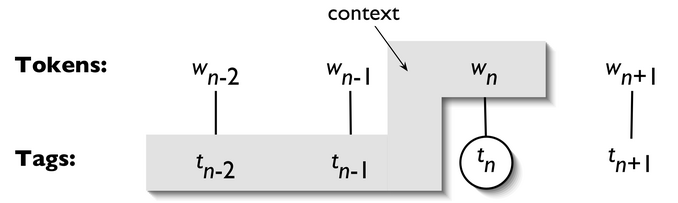
\includegraphics[width=0.4\textwidth]{tag-context.png} 
\end{center}
\caption{Tagger Context}
\label{fig:trigram}
\end{figure}

The tag to be chosen, $t_{n}$, is circled, and the context is shaded in grey.
In the example of an n-gram tagger shown in figure \ref{fig:trigram}, we have $n=3$; that is, we consider the tags of the two preceding words in addition to the current word.
An n-gram tagger picks the tag that is most likely in the given context.
\par
Altrough we use the name trigram all throughtout this paper, we acctually refer to sequential tagger, which consists of
\textit{affix}\footnote{The Affix tagger learns prefix and suffix patterns to determine the part of speech tag for word.}, \textit{unigram}, \textit{bigram} and \textit{trigram} taggers in this order respectively. First we build affix, which is used as ad \textit{backoff-tagger} for unigram. Unigram is afterwards used as a backoff-tagger for bigram, which is finally used for trigram.

\subsection{Brill tagger} %BANIČ
\textit{TODO - BANIČ}
Banič glej ta link : nltk.googlecode.com/svn/trunk/doc/book/ch05.html
poglavje 5.6
\subsection{Naive Bayes tagger} %BANIČ
\textit{TODO - BANIČ}

\section{Related work}
\subsection{Nltk-trainer} %NIKICC
The code for building the tagger was taken from \textit{Nltk-trainer}  project \cite{nltk-trainer}, whose author is Jacob Perkins.
Its an open-source project hosting on Github, with moto to \textit{Train NLTK objects with zero code}.
We almost exclusively used the script \texttt{train\_tagger.py}, which has the ability to generate NLTK taggers. The 

\subsection{JOS corpus} %BANIČ
The basic component for building Slovene tagger is \textbf{JOS corpus} from JOS project \cite{JOS}. It stands for: \textit{Jezikoslovno Označevanje Slovenskega jezika} (Linguistic annotation of Slovenian language).
It contains collections of various text in Slovenian language with annotation.
For our project we used jos1M corpus that contain 1 million words with it's appropriate lemmas and morphosyntactic descriptions.
The JOS is compatible with Slovene\textit{ MULTEXT-East morphosyntactic specifications Version 4}\cite{MULTEXT-East}.
It basic purpose is to define word classes.
For each class there are various attributes and their appropriate values, which they can be mapped into morphosyntactic descriptions (i.e. MSD).
The structure of JOS corpora is in  \textbf{Extensible Markup Language (XML)}.

\section{Implementation}
\subsection{Corpus transformation} %BANIČ
\label{Corpus transformation} 
\textit{TODO - BANIČ}\\
We can easily manipulate XML files in various programming languages (e.g. Python with xml.dom.minidom).
This is mandatory because \textit{nltk-trainer}\cite{nltk-trainer} expects special form of input file.
For further information see \ref{Corpus transformation}.

\subsection{Training the tagger} %NIKICC
As mentioned above, the script \texttt{train\_tagger.py} was used for this pupose. Its mandatory argument is a corpus in .pos format, which generation is described in \ref{Corpus transformation}. Beside this, there are many optional arguments. Here we will describe basics, for further description run script help with
\begin{lstlisting}
train_tagger.py --help
\end{lstlisting}
\par
One is wheather to generate a Sequential Tagger, a Brill Tagger or a Classifier Based Tagger. For Sequential we can then select sequential backoff algorithm. This can be any combination of the following letters:
\begin{itemize}
\item a: AffixTagger
\item u: UnigramTagger
\item b: BigramTagger
\item t: TrigramTagger
\end{itemize}
The default is \textit{aubt}, which was used for our Trigram tagger, but you can set this to the empty string to not train a sequential backoff tagger. The Brill Tagger is trained in front of the other tagger, which in our implementation was the Trigram tagger. When building classifier based algorithm, we must select the classifier or the sequence of classifier. Following are supported: NaiveBayes, DecisionTree, Maxent, GIS, IIS, CG, BFGS, Powell, LBFGSB, Nelder-Mead, MEGAM and TADM. We should mention, that the time spent for training classifier based tagger, is much larger than, the time for a sequential or brill.
\par
Script also has the possibility to set default tag. We used \textit{-Neznan-}, which is Slovene word for \textit{-unknown-}.
\par
Last argument, that should be mentioned, is wheather to evaluate the tagger or not and the procentage of sentaces to be used. The default value is 1, which means that the \textit{same} sentances are first used for training the tagger and then for evaluation. We reccomend this argument to be set below 1. If so, the right approach is used.
Sentances are devided into two groups, one in used for training and second for evaluation. \textit{Fraction} is the procentage of sentances assigned to training group. 
This was used for evaluating constructed taggers. For results of this evaluation see section \ref{results}).

\subsection{Usage with NLTK} %BANIČ
\textit{TODO - BANIČ}
\subsection{Encoding problems} %BANIČ
\textit{TODO - BANIČ}

\section{Results} %NIKICC
\label{results}
For all constructed taggers, we here provide their accuracy. The results were obtained by repeating the proces of building the tagger with various evaluation arguments. See table \ref{tab:evaluation} and figure \ref{fig:evaluation}.

\begin{table}[htb]
\begin{center}
\begin{tabular}{c|c|c|c}
\textit{fraction} & \textit{Trigram} & \textit{NaiveBayes} & \textit{Brill} \\\hline\hline
0.75  &  0.8286  &  0.8451  &  0.8490\\
0.80  &  0.8304  &  0.8461  &  0.8514\\
0.82  &  0.8306  &  0.8465  &  0.8515\\
0.84  &  0.8299  &  0.8462  &  0.8508\\
0.86  &  0.8306  &  0.8472  &  0.8512\\
0.88  &  0.8299  &  0.8474  &  0.8517\\
0.90  &  0.8288  &  0.8467  &  0.8507\\
0.91  &  0.8278  &  0.8462  &  0.8489\\
0.92  &  0.8276  &  0.8464  &  0.8490\\
0.93  &  0.8281  &  0.8464  &  0.8491\\
0.94  &  0.8278  &  0.8461  &  0.8496\\
0.95  &  0.8289  &  0.8475  &  0.8510\\
0.96  &  0.8388  &  0.8538  &  0.8609\\
0.97  &  0.8401  &  0.8568  &  0.8612\\
0.98  &  0.8417  &  0.8588  &  0.8629\\
0.99  &  0.8379  &  0.8567  &  0.8578\\\hline\hline
\textit{average} & \textbf{0.8317} & \textbf{0.8490} & \textbf{0.8529}
\end{tabular}
\end{center}
\caption{Taggers accuracy for various fractions.}
\label{tab:evaluation}
\end{table}

\begin{figure}[htb]
\begin{center}
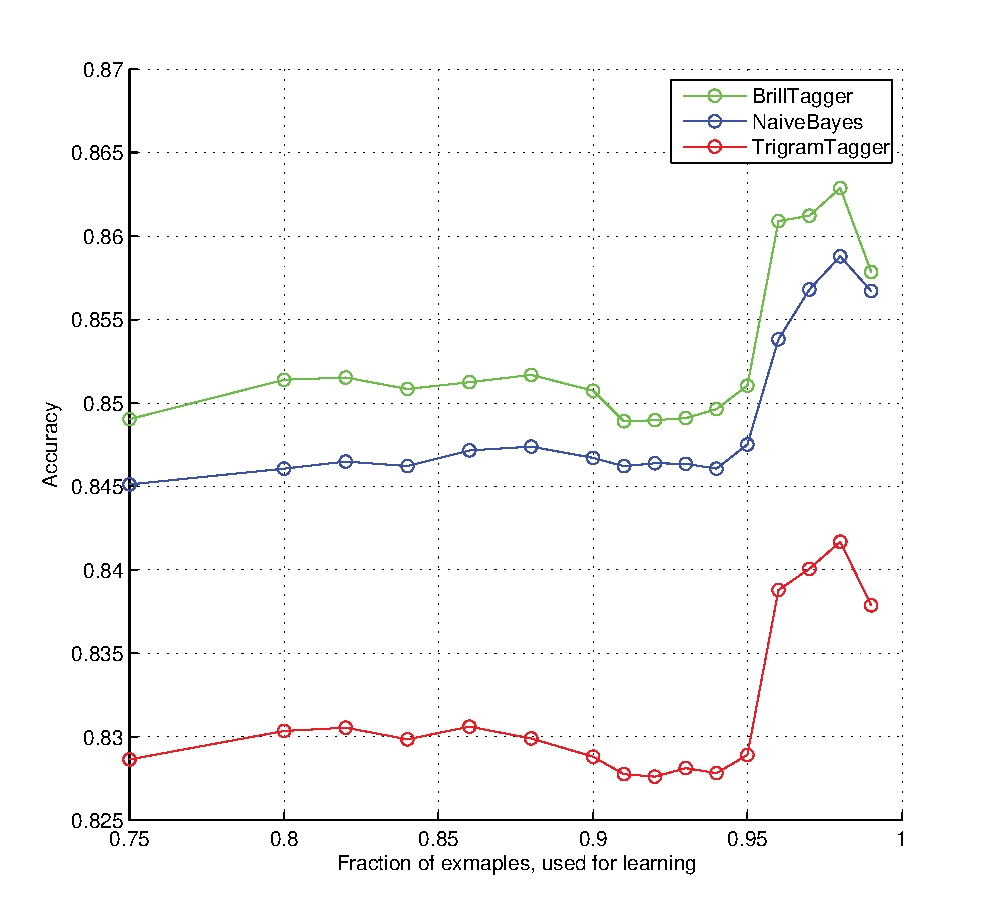
\includegraphics[width=0.5\textwidth]{../evaluation/graph.pdf} 
\end{center}
\caption{Accuracy evaluation results.}
\label{fig:evaluation}
\end{figure}
\par
To conclude, there are no major differences in tagging accuracy. The Brill and the Naive Bayes are about 2\% better than Trigram.
\par
However, during this evaluation we discover an other paramater, which should be taken into account.
Under the assumption that most of the time was actually spent for tagging the sentances (besides just testing for equallity and percentage calculation are needed), we noticed that the time for evaluations differ drastically.
The results of resarching time consumption are listed in table \ref{tab:evaluation_speed} and graphically represented on figure \ref{fig:evaluation_speed}.

\begin{table}[htb]
\begin{center}
\begin{tabular}{c|c|c|c}
\textit{number of words} & \textit{Trigram} & \textit{NaiveBayes} & \textit{Brill} \\\hline\hline
   50  &  0.0003 &   4.1543  &  0.0011\\
   75  &  0.0004 &   6.2464  &  0.0014\\
  100  &  0.0006 &   8.5232  &  0.0018\\
  125  &  0.0008 &  10.6370  &  0.0020\\
  150  &  0.0009 &  12.4937  &  0.0024\\
  175  &  0.0011 &  14.5484  &  0.0027\\
  200  &  0.0011 &  16.3944  &  0.0029\\
  225  &  0.0013 &  18.6332  &  0.0032\\
  250  &  0.0015 &  20.7357  &  0.0035\\
  275  &  0.0017 &  22.8280  &  0.0041\\
  300  &  0.0018 &  24.8243  &  0.0042\\
  325  &  0.0018 &  27.4270  &  0.0043\\
  350  &  0.0022 &  29.2458  &  0.0051\\
  400  &  0.0023 &  32.9599  &  0.0052\\
  425  &  0.0024 &  36.0322  &  0.0056\\
  450  &  0.0027 &  38.1471  &  0.0062\\
  475  &  0.0027 &  39.2278  &  0.0064\\
  500  &  0.0029 &  41.2688  &  0.0063\\
\end{tabular}
\end{center}
\caption{Time spent in seconds for tagging different numbers of words.}
\label{tab:evaluation_speed}
\end{table}

\begin{figure}[htb]
\begin{center}
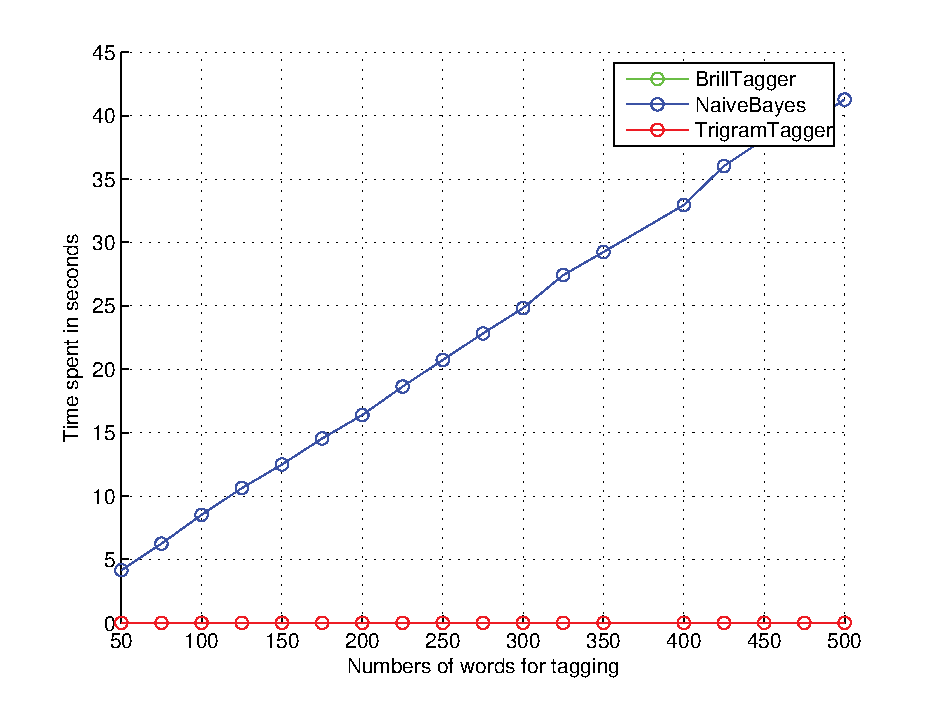
\includegraphics[width=0.5\textwidth]{../evaluation/graph_speed.pdf} 
\end{center}
\caption{Spent time measurements. NOTE: The green line is not visible because it is right under the red one.}
\label{fig:evaluation_speed}
\end{figure}

The difference here is enormous. Brill and Trigram run at almost the same speed, while Naive Bayes runs extremely slower.

\section{Conclusion} %BANIČ
\textit{TODO - BANIČ}

\section*{Acknowledgements}
We would like to express our our gratitute to all the contributor of \textit{JOS} \cite{JOS} and  \textit{nltk-trainer} \cite{nltk-trainer} projects and out mentor at Faculty of Computer and Information Science.

\begin{thebibliography}{99}
\bibitem{JOS} \url{http://nl.ijs.si/jos/}
\bibitem{nltk-trainer} \url{https://github.com/japerk/nltk-trainer}
\bibitem{MULTEXT-East} \url{http://nl.ijs.si/ME/V4/msd/html/msd-sl.html}
\bibitem{NLTKBOOK} \url{http://www.nltk.org/book}
\end{thebibliography}
\end{document}